%%%%%%%%%%%%%%%%%%%%%%%%%%%%%%%%%%%%%%%%%%%%%%%%%%%%%%%%%%%%%%%%%%%%%%%%%%%%%%%
%
%               LaTeX-Template for theses at the PST group.
%
% Authors:
%       Matthias Hölzl/Moritz Hammer, 2006
%       Annabelle Klarl 2011
%%%%%%%%%%%%%%%%%%%%%%%%%%%%%%%%%%%%%%%%%%%%%%%%%%%%%%%%%%%%%%%%%%%%%%%%%%%%%%%

\documentclass{thesisPST}
% macros for theses at the PST group
% 
% Matthias Hölzl, 2006
% Annabelle Klarl, 2011

\usepackage{listings} % source code printer package

% for code snippets -> see also http://www.ctan.org/tex-archive/macros/latex/contrib/listings/listings.pdf
\lstnewenvironment{pseudocode}[1][]
{\lstset{
	language=Java,
	tabsize=3,
	mathescape=true,	
	frame=single,
	framexleftmargin=5mm,
	xleftmargin=0cm,
	%aboveskip=,
	%belowskip=,
	%backgroundcolor=\color{yellow},
	escapeinside='',
	showstringspaces=false,
	captionpos=b,
	numbers=left,
	numberstyle=\tiny,
	stepnumber=1,
	numbersep=5pt,
	%firstnumber=100
	basicstyle=\footnotesize\ttfamily,
	keywordstyle=\bf,
	morekeywords={},
	deletekeywords={},
	identifierstyle=,
	commentstyle=\color{grey},
	escapechar=§
	}
}{}

\usepackage{wrapfig}
\usepackage{eurosym}

\begin{document}

%%%%%%%%%%%%%%%%%%%%%%%%%%%%%%%%%%%%%
%% Change according to your thesis %%
%%%%%%%%%%%%%%%%%%%%%%%%%%%%%%%%%%%%%
% change according to your thesis (german or english!)
\thesisType{Bachelor Thesis} 
\thesisAuthor{Jonas Kemper}
\thesisProgram{Medieninformatik Bachelor}

\thesisTitle{MicroPsi and Minecraft}

% Do not delete this command!
% If you do not have a a subtitle, leave it empty!
\subtitle{A Popular Video Game as a Simulation Environment\\
 for a Cognitive Architecture}

\referee{Prof.~Dr.~Martin Wirsing}
\supervisor{Joscha Bach~PhD, Annabelle Klarl}

\handInDate{19. September 2013}

%\selectlanguage{ngerman}
\selectlanguage{english}

% use this command to define syllable division for special words (e.g. class names)
\hyphenation{Be-ant-wortung}
\hyphenation{-Mo-di-fi-ka-tio-nen}
\hyphenation{Open-GL}

%%%%%%%%%%%%%%%%%%%%%%%%%%%%%%%%%%%%%
%%%%%%%%%%%%%%%%%%%%%%%%%%%%%%%%%%%%%

\frontmatter % for Roman numbering 
\maketitlepage
\cleardoublepage
\selbststaendigkeitserklaerung
\cleardoublepage
\pagestyle{headings}

%%%%%%%%%%%%%%%%%%%%%%%%%%%%%%%%%%%%%
%% Change according to your thesis %%
%%%%%%%%%%%%%%%%%%%%%%%%%%%%%%%%%%%%%

\chapter*{\centering \begin{normalsize}Zusammenfassung\end{normalsize}}
\begin{quote}


Simulationsumgebungen spielen für das Testen und Erforschen von neuen Ansätzen für künstliche Intelligenz eine entscheidende Rolle. Da sich Computerprogramme nur mit erhöhtem technischen und finanziellen Aufwand in die physische Welt implementieren lassen, können simulierte Umgebungen schnellere, günstigere und reproduzierbarere Ergebnisse liefern. Genauso wie Innovationen aus dem Bereich der KI neue Impulse setzen, können auch neue Ansätze für Simulationsumgebungen zu neuen Erkenntnissen führen.

Das populäre Videospiel Minecraft bietet sich durch die kompositionale Semantik der Spielwelten besonders als Grundlage für eine Simulationsumgebung an, da das Agentensystem durch das Erforschen seiner Umwelt, Wissen über die Spielwelt aufbauen und sich ähnelnde Strukturen wiedererkennen kann. Objekte der Spielwelt sind in Minecraft keine bloßen Hindernisse, sondern werden mit variablen Eigenschaften prozedural generiert. Durch die Komposition dieser Objekte entstehen Umgebungen, die einer realen Umgebung in dieser Hinsicht eher gleichen, als andere virtuelle Welten. Da Minecraft einen umfangreichen Mehrspielermodus beinhaltet, lässt es sich zudem für Multiagenten-Umgebungen und so für Simulationen mit kollaborativen Agenten verwenden. Darüber hinaus sind Minecraft-Lizenzen günstig zu erwerben, erhältlich für viele Plattformen und es gibt eine äußerst große und aktive Community für selbsterstellte Spiel-Inhalte und Modifikationen.

Diese Arbeit präsentiert eine Schnittstelle, welche es der kognitiven Architektur MicroPsi 2 ermöglicht, sich an einem Minecraft Server anzumelden, die Umgebung wahrzunehmen und sich darin fortzubewegen. Im Anschluss daran wird die Visualisierungskomponente vorgestellt, welche eine mit Open-GL gerenderte 3D-Ansicht der Simulationsumgebung live im MicroPsi 2 User Interface anzeigt. Es folgt die Beschreibung eines einfachen Experimentes, bei welchem sich ein Agent selbstständig auf ein vorher definiertes Objekt zubewegen muss. Die Arbeit endet mit der Dokumentation und Auswertung des Experimentes.\end{quote}

\chapter*{\centering \begin{normalsize}Abstract\end{normalsize}}

\begin{quote}

Simulation environments play an important role for testing and researching new approaches to artificial intelligence. Because computer software can only be implemented into the physical world with increased technical and financial effort, simulated environments can deliver results faster, cheaper and more reproducible. In the same way as innovations in AI can deliver new impulses, new approaches to simulation environments can just as well lead to new insights into the future of intelligent machines.

Because of its compositional semantics, the popular video game Minecraft turns out to be an interesting simulation environment, as agents can generate knowledge through exploring their environment and recognising similar structures. Objects in Minecraft worlds are not just obstacles, but are generated procedurally with varying characteristics. Through composition of these objects, environments emerge that in this aspect are more similar to real environments than other virtual worlds. Since Minecraft contains an extensive multiplayer mode, it is also suitable for multi-agent environments and for simulations with collaborative agents. Furthermore, Minecraft licenses are affordable and available for many platforms and there is a huge and active community for player generated content and modifications.

This thesis presents an interface which enables the cognitive architecture MicroPsi 2 to connect to a Minecraft server, perceive its environment and move around within it. Subsequently, the visualisation component is introduced that displays an OpenGL rendered 3D view live in the Micro Psi 2 user interface. It is followed by the description of a simple experiment in which the agent has to move towards a previously specified object. The thesis concludes with the documentation and evaluation of the experiment.
\end{quote}
% change according to your thesis 
% german: Danksagung
% english: Acknowledgements)
\chapter*{\centering \begin{normalsize} Acknowledgements\end{normalsize}}
I would like to thank Prof. Dr. Martin Wirsing for giving me the opportunity to prove my motivation in writing a thesis about what I considered would suit me best. I thank my supervisor Joscha Bach, for giving me the opportunity to work with his creation, advising and inspiring me through the entire process.
I especially thank my supervisor Annabelle Klarl, for supporting my plan without hesitation, guiding me through the process and providing valuable feedback whenever I needed it. Dominik Welland helped me with understanding and building upon the MicroPsi framework and fixed inhabitant bugs as soon as I reported them, thank you!

Additionally I would like to thank Michael Fogleman whose code I built upon and especially Nick Gamberini who allowed me to use his Spock for this project and who answered every question about it in detail. Finally, I thank all the other members of the Minecraft community, who collect and distribute structured knowledge regarding the game in a combined effort and have answered my questions about the game and how it works in IRCs and message boards.

%%%%%%%%%%%%%%%%%%%%%%%%%%%%%%%%%%%%%
%%%%%%%%%%%%%%%%%%%%%%%%%%%%%%%%%%%%%

\cleardoublepage
\tableofcontents

\mainmatter % for Arabic numbering

%%%%%%%%%%%%%%%%%%%%%%%%%%%%%%%%%%%%%
%% Change according to your thesis %%
%%%%%%%%%%%%%%%%%%%%%%%%%%%%%%%%%%%%%
\chapter{Introduction}
The hunt for artificial intelligence started many years ago. Dividing the subject into the strong and the weak part means separating its goals into useful applications and those that try to learn about the nature of intelligence itself. The ultimate task of strong AI---recreating human intelligence---admittedly still seems to be science fiction, though.

But then again: a new generation of cognitive scientists, psychologists and computer scientists strives to implement new ideas for simulated cognition by building cognitive architectures. Many of them do so by simulating, in one way or the other, what we would call neural node nets.

One of these architectures is MicroPsi 2. Developed by Joscha Bach and Dominik Welland, it is based on the Psi theory by Dietrich Dörner, who is a German professor for theoretical psychology. It aims at providing a solid and complete implementation of his theory of cognition and at the same time at being easily accessible, understandable and modifiable for the research and applications to come.

To test the functionality of such cognitive architectures and to figure out their capabilities and potential, we need to research their behaviour inside defined environments. As implementing AI into the physical world (as robots, for example) requires building appropriate hardware and patience, computer-simulated environments, therefore, play an important role.

MicroPsi 2 is both: a cognitive architecture as well as a set of and an interface to simulation environments.

\section{Motivation}
Video games are natural applications of artificial intelligence. The quality of a games AI can make all the difference in between an immersive experience and an uninspired demonstration of computer graphics technology. One game that especially stood out in the recent years is Minecraft. As a so called \emph{sandbox game}, it attempts to leave the player with as few limitations as possible, for what they do and how they behave in the game world. This kind of relatively open world delivers a simulated environment rich of opportunities, for both human and artificial players. Building an interface in between the cognitive architecture MicroPsi 2 and the video game Minecraft is what this thesis is about.


\section{Outline}
This project is fundamentally about combining existing technologies. The most important ones being MicroPsi 2, the most ambitious framework aiming to implement the ideas of the Psi theory, and Minecraft, the popular sandbox videogame.

To understand how and why they were chosen, a brief history of their creation as well as explanations of their basic ideas and relevant insights into their architecture are given in chapter two and three. Chapter two introduces the Psi theory and its implementations. We will especially focus on the particular implementation MicroPsi 2 and describe its modules in detail. Chapter three introduces the video game Minecraft, its protocol and related software projects. As the resulting software heavily relies on them, the protocol and the utilized open source software will get increased attention. 
In Chapter four the contribution of this thesis, the Minecraft world adapter for MicroPsi 2, is being described in detail. As a proof of concept, the description eventually leads to a small experiment.
Chapter five summarises the findings of this thesis and gives an outlook on possible future applications.

%TODO Zuviele Kommas ;), im Englischen werden so gut wie keine Kommas verwendet!

%TODO !!!! Sehr wichtig wäre die Überarbeitung der AIG Kapitels. Ich habe gar nicht verstanden, um was es in der Psi Theorie geht und deswegen natürlich auch nicht die Implementierung dazu. Das zieht sich dann auch durch in deine Implementierung und die Case study. Hier empfehle ich dir dringend eine ausführlichere Erklärung!

\chapter{Artificial General Intelligence}
\label{chap:2}
To provide the necessary context for this thesis, this chapter will provide a brief introduction to the corresponding foundations on the AI side.

%TODO !! was ist strong AI? Du kannst nicht davon ausgehen, dass der Leser das weiß

First, we will introduce AIG as a subset of artificial intelligence. Based on this, the Psi theory, as a particular instance of strong AI theories, is described in detail. The description includes a brief history of its concrete implementations. Then, MicroPsi~2, the latest framework dedicated to the Psi theory, is described in detail.

    \section{Strong AI}
    
%TODO Den Satz versteh ich nicht    
    
It took many years for AI research to evolve from the early ideas of thinking machines over Deep Blue, the computer that could beat mankind's best chess players to Watson, the AI that beats the champions of Jeopardy, the game show, that is about asking the appropriate question to a given answer. There exist many applications for AI. Self-driving cars and online-shopping recommendation systems to name a few.

%TODO Zitierung der Quelle der Definitionen?

These examples have one thing in common. They are applications of technology that serves an immediate, or at least foreseeable purpose. For AI in scenarios of this kind, the term \emph{applied AI} (or \emph{weak AI}) has been coined. \emph{Strong AI}, in contrast, is about researching the nature of intelligence itself. An actual (hypothetical) implementation of a strong AI would mean, one would have to build a machine, that is capable of acting like a human being---not just for a limited problem set, but in all of them. 

%TODO feelings? really?

Another term, that is being used more recently, is \emph{AIG}, for \emph{Artificial General Intelligence}. It it is in contrast to what are called \emph{narrow AI} applications, which chess computers and other expert systems would be an excellent example for. AIG sets out, to develop software that can solve and act appropriately in a wide variety of problem fields, without specialising on any particular problem whatsoever. A complete AIG system is supposed to control itself autonomously and to have it's own thoughts and feelings. This has been the original focus of the AI field, before many lost their enthusiasm about it, when it turned out being not as imminently as expected. Even though the advances in narrow AI contribute to it, AIG is more than just an assembly of these. There is a huge number of different AIG projects being worked on, with most of them being in early stages.~\cite{goertzel2007artificial}

%TODO Was ist der Unterschied zwischen strong AI und AIG?

%TODO Versteh ich nicht

Cognitive AI, in particular, can be thought of as architectures that implement findings and theories in the fields cognitive science and psychology, as well as the neurosciences, for the sake of proving, if the theories hold against what they promise. Many cognitive architectures share characteristics with or directly implement artificial neural networks.

%TODO Sollte das nicht bei der Definition von weak und strong AI kommen? Warum erst jetzt? Wieso springst du immer zwischen den Bezeichnungen strong AI and AIG hin und her?

Looking upon the field of AI from a philosophical point of view, computers seem to deliver enormous potential for learning about how minds work. At the same time, new questions arise. If we knew how cognition works and if we could build machines that simulate it, would these minds be real? And what would the ethical implications be? According to Russel's and Norvig's standard reference \emph{Artificial Intelligence: A Modern Approach}~\cite{russell2009artificial}, one can distinguish in between two fundamental assumptions. The assumption that computers are able to act \emph{as if} they were intelligent is called the weak AI hypothesis. Thinking that an intelligently acting machine ,in fact, \emph{is} performing cognition, is called strong AI hypothesis.

Putting it differently, weak AI considers computers to be an instrument to research cognitive processes, whereas strong AI considers simulated cognitive processes as actually being cognition.

%TODO Ab hier ist mir nicht ganz klar, warum du das alles schreibst. Ist schön zu lesen, aber ich erkenne den Beitrag zu deiner Arbeit nicht. Außerdem wirst du hier sehr emotional ;)

Trying to figure out, if machines are able to achieve cognition, we often explain by enumerating things that computers can not to. They can not be kind, friendly or have a sense of humour. Neither can they tell right from wrong, fall in love or learn from experience. But what can they do? They are at least partly involved in almost every significant recent discovery in most sciences. They steer cars safer than we ever did. Where \emph{exactly} to draw the dividing line between intelligence and machinery?~\cite{russell2009artificial}

The most famous indicator for whether a machine is intelligent or not, is the Turing test. Decades after its formulation, contests regarding to it are still being held---may the best conversationalist win! Many would argue that even an algorithm that passes the Turing test would still not be intelligent. It would trick people into thinking it was, but it would still not be conscious, aware of itself. Moreover, it would not have emotions.~\cite{russell2009artificial}

But, would not what we believe is possible and what is not, become obsolete, once we would be able to build something that cognition can not be denied from? 

Eventually, this question, might not be as significant as it appears to be. Dijkstra tried to explain that whether something is able to think or not, is first and foremost a matter of language and the interpretation of the word \emph{think}, when he famously said: ``The question of whether machines can think... is about as relevant as the question of whether submarines can swim.''

    \section{Psi Theory}
    
%TODO !! cite! Originalzitat sehr wichtig!

This section gives an overview of the basic ideas of the Psi theory. The descriptions are based on \emph{Principles of Synthetic Intelligence PSI: An Architecture of Motivated Cognition}~\cite{Bach:2009:PSI:1611304} by Joscha Bach.

The theory in its foundations was first described by German psychologist Dietrich Dörner in his books ``Bauplan für eine Seele''~\cite{Doerner1998} and ``Die Mechanik des Seelenwagens''~\cite{dorner2002mechanik} from 1998 and 2002. Dörner's holistic approach goes beyond classic problem solving and develops a unified model for cognition that implements motivation and emotions. He is convinced that artificial intelligence does not have to focus on different aspects of cognition that have to be looked at separately but that a unified theory will ultimately lead to a deeper understanding of cognition itself.
    
Dörner's ``Bauplan für eine Seele''~\cite{Doerner1998} (``blueprint for a mind'') belongs in the interdisciplinary field Cognitive Science, as with his theory he tries to research psychological foundations with the methods of Computer Science. The theory is an attempt to explain the mind as a machine. It has a notable focus on the emotional system and addresses symbolic and sub-symbolic reasoning.  The mind is looked at as a fuzzy and self-extending causal network structure.

The theory tries to model the human mind as an agent, that is controlled by a structure of relationships and dependencies, that strives to maintain homeostatic balance. Every form of representation of the agent's cognition---may it be percepts, plans or abstractions of space and objects---are represented as directed, hierarchic spreading-activation networks. This structure can be visualised as an artificial neural network, which we will call \emph{node net} in the following. Nodes in these networks have gates that may send activation and slots that may receive it. The basic elements a node net consists of are called \emph{quads}. Quads themselves consist of one central neuron and four outer neurons that are called \emph{sub}, \emph{sur}, \emph{ret} and \emph{por}~(see figure~\ref{quad}). The outer neurons can be connected with the central neurons of other quads and thereby form networks. The four different kinds of outer neurons represent different kinds of relations. \emph{sub} stands for a ``has part'' relationship, \emph{sur} is the inverse to sub an represents an ``is part'' relationship, \emph{ret} stands for the ordering relationship of succession and \emph{por} represents predecession.

\begin{figure}[h]
  \centering
    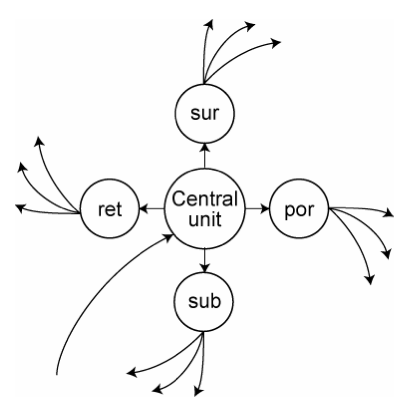
\includegraphics[width=6cm]{graphics/quad}
  \caption{Quads like this are the basic representational unit of the Psi theory (taken from \cite{Bach:2009:PSI:1611304})}
  \label{quad}
\end{figure}

Furthermore each neuron has an activation value, that it receives from and forwards to other neurons. Links in between neurons can be modified to dynamically modulate the forwarded activation value. The modulation of the flow of activation is interpreted as emotions.

There are specific kinds of neurons that are called \emph{sensors} and \emph{actuators}. They represent the in- and output to the outside world. Sensors receive activation if they are triggered by the environment and activated actuators lead to an action in the environment.

The motivation of Psi agents comes from a set of predefined drives. They are divided into physiological (e.g. physical integrity), social (e.g. affiliation) and cognitive drives (e.g. reduction of uncertainty). These drives may signal a specific demand. If the value of a demand changes, pleasure or displeasure signals are sent to the agent. By reinforcement learning agents learn what behaviour leads to the fulfilment of demands. 

As node nets may create new nodes and links on their own, the agent forms memory, motives and plans, that help it to select what action to execute next (see figure~\ref{motive_architecture}). Agents can store representation of their entire percept sequence, but only those that are connected to pleasure or displeasure signals are being kept.

\begin{figure}[h]
  \centering
    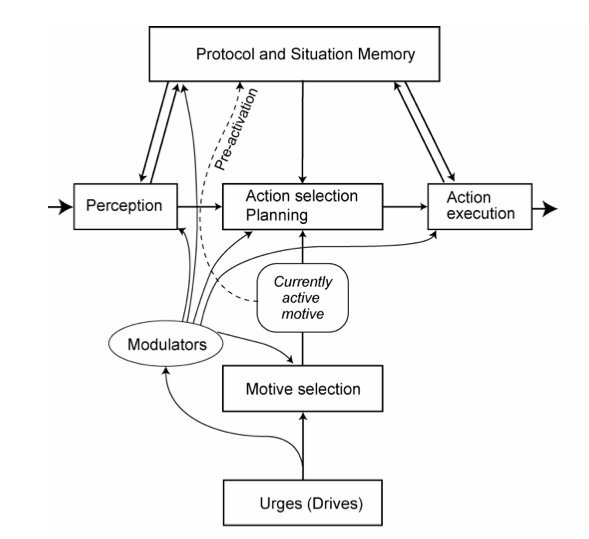
\includegraphics[width=10cm]{graphics/motive_architecture}
  \caption{The basic architecture of action selection in Dörner's theory (taken from \cite{Bach:2009:PSI:1611304})}
  \label{motive_architecture}
\end{figure}

Quads are used to form \emph{partonomies} that represent information about concepts and relationships. A partonomy is a hierarchical structure that represents a part-whole relationship. For example, the concept ``head'' would be represented as the assembly of a face and a head. A face furthermore would itself consist of a mouth, a nose, eyes and so forth~(see figure~\ref{partonomy}). 

Through the combination of partonomies and order relations, all basic types of relationships the agent stores are formed. These could be causal, spatial or temporal relationships in between states of the environment, for example.

\begin{figure}[h]
  \centering
    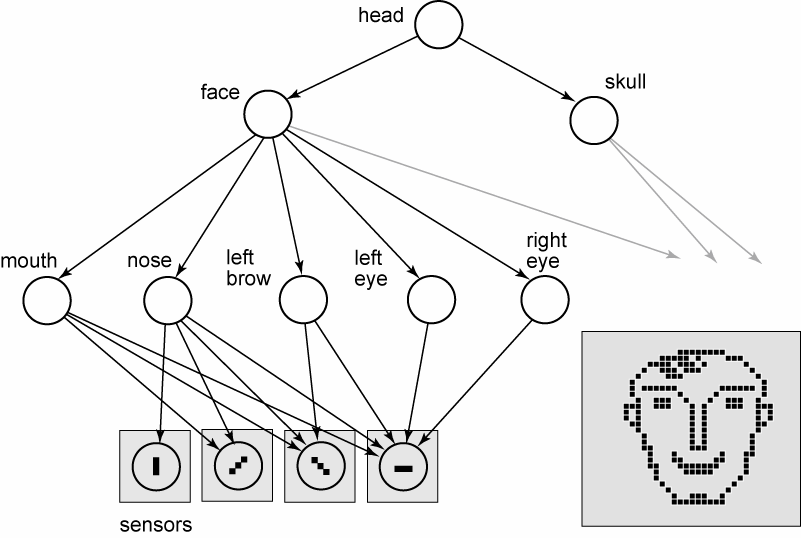
\includegraphics[width=9cm]{graphics/partonomy}
  \caption{The partonomic representation of a Cartoon face (taken from \cite{Bach:2009:PSI:1611304})}
  \label{partonomy}
\end{figure}

Psi agents' basic approach to problem solving works by going through a set of subsequent stages. The agent first tries to approach a problem with behavioural routines. If these do not solve the problem, the agent tries to construct a plan, by trying to find a chain of causal relationships that ultimately lead to a state, that solves the problem. If no plan is found, the agent starts to explore its environment to gather more knowledge.

The goal of implementing the theory to computer software is to find potential inconsistencies and moreover to find out if Psi agents show similar behaviour to that of humans. If they do, the Psi theory could possibly serve as an explanation about how human minds work. For this purpose, a number of experiments---similar to video games---have been concluded, in which both Psi agents and human players had to perform specific tasks. Later on, their behaviours have been compared and searched fir similarities and differences.
 
%TODO !!! Das ist deine Hauptgrundlage!!! Ich habe leider nicht verstanden,was die Grundgedanken sind. Du musst die Grundkonzepte der Theorie vorstellen und in Relation setzen. Was ist die Motivation für die Theorie, was erreicht man damit, wie erreicht man die Ziele? Abbildungen tragen sicherlich auch zum Verständnis bei!

Joscha Bach adapted the theory to bring it in a contemporary form with slight modifications in his dissertation \emph{Principles of Synthetic Intelligence PSI: An Architecture of Motivated Cognition}~\cite{Bach:2009:PSI:1611304}. Even though building a conscious machine that thinks and acts as we do is still mere science-fiction, it is this kind of foundational research, that leads us to new ways of thinking about the world, that give us our most significant leaps.
    
    \section{Agents and Environments}

%also define symbolic and subsymbolic    

Before we continue to describe concrete implementations and simulations, we define agents and environments according to Russel and Norvig.~\cite{russell2009artificial} 

%TODO Ist das ein wörtliches Zitat? Ist besonders zu kennzeichnen!

An \emph{agent} is defined as anything that can perceive its environment through sensors and conduct actions inside the environment through actuators. The examples given in \cite{russell2009artificial} include a software agent that may receive network packets as sensory inputs and produces output by writing files and sending network packets fits in nicely within this thesis. However, agents can just as well be robots that have cameras as sensors and motors as actuators. Even humans can be thought of as agents that perceive their environment through their senses and act upon it through their muscles.

Russel and Norvig furthermore define the \emph{percept}, as the agent's input and the \emph{percept sequence} as the complete history of what the agent has perceived. Each decision an agent makes is based on the percept sequence.

Additionally, they describe the \emph{agent function}, as the function that maps each percept sequence to an action. The \emph{agent program} is its concrete implementation.

A \emph{rational agent} is an agent that acts appropriately to any given percept sequence. To answer the question about what is appropriate and what is not, they introduce \emph{performance measures} that evaluate the agent's actions. These measures have to be defined by the designer of an experiment. Summarising, the rational agent tries to maximise its performance measure at any given point of time.

%TODO Ich frage mich, ob diese Definitionen alle nötig sind. Du solltest später dann darauf eingehen, wie deine konkrete Implementierung im Bezug auf diese Definitionen zu sehen ist.

\emph{Environments} have a number of different properties. They can either be \emph{fully observable} or \emph{partially observable}. An environment is fully observable when the agent has access to the complete state of the environment---or at least to everything that is relevant, regarding to the performance measure. As opposed to this, it is partially observable, if the previously mentioned requirement is not given.

An environment can moreover be \emph{single agent} or \emph{multiagent}. An environment is multiagent, when there is at least one other agent, whose behaviour is about maximising a performance measure that depends on the first agent's behaviour. If the agents try to maximise the performance measure of all agents, the environment is called \emph{cooperative}. If agents try to maximise their own and minimise the performance measure of the other agents, it is called \emph{competitive}.

An environment may furthermore be \emph{discrete} or \emph{continuous}. If an environment can be thought of as advancing from one discrete state to the other, it is discrete (and even more so if there is a finite number of states). If the transitions between states are thought of as being continuous, so is the environment.

A \emph{task environment} is the combination of the performance measure, the environment and the agent's actuators and sensors.

    \section{Psi Implementations}
Psi has been implemented by different groups at different times. The first implementations are by Dörner and his associates themselves~(see figure \ref{psi_screen}). They used Delphi Pascal and developed it for Windows environments. This implementation can still be downloaded (\cite{PsiDownload}) and runs on Windows 7 installations, for example. 

\begin{figure}[h]
  \centering
    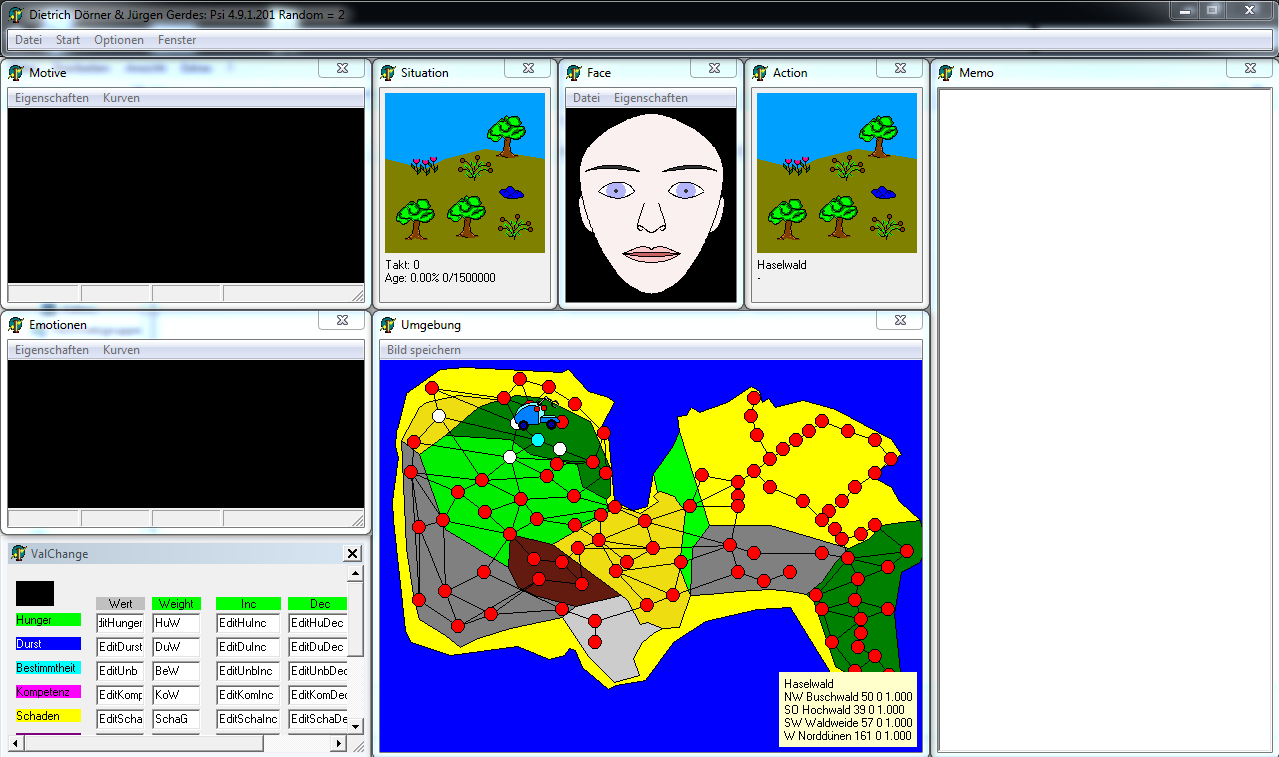
\includegraphics[width=10cm]{graphics/psi_screen1}
  \caption{Screenshot of Dörner's team's Delphi Pascal Psi implementation}
  \label{psi_screen}
\end{figure}

%TODO Was ist das? Vorher nie erwähnt!

Subsequently, there has been a simple 3D implementation of Dörner's island simulation called Psi3D.

%TODO was bedeutet "interfacing the world"?

The work on Dörner's team's implementations has not been continued, so Joscha Bach and his associates developed new implementations of Psi. From 2003 to 2009 they built an implementation in Java as a set of plugins for the Eclipse IDE called MicroPsi. It included a graphical editor and a broad experimentation framework. MicroPsi provided a complex and sophisticated simulation component which contained simulated objects in three dimensional worlds---even though most experiments took place on a plane. As a pragmatic approach, different ground types of the simulation world have been stored in bitmap files similar to height-maps. The framework offered complex administrator interfaces and appealing DirectX rendered 3D-views of the scenery as well as a more general world view which interfaced the world by providing clickable objects. Predefined simulation environments included a classic Island and a Mars world (see figure~\ref{micropsi_3d_screen}). Objects in these worlds may be assembled recursively out of other objects and bring their own functionalities. As it has been the case in Dörner's implementation, a viewer for facial expressions has been included---this time as well as a three-dimensional simulation.~\cite{Bach:2009:PSI:1611304}


\begin{figure}[h]
  \centering
    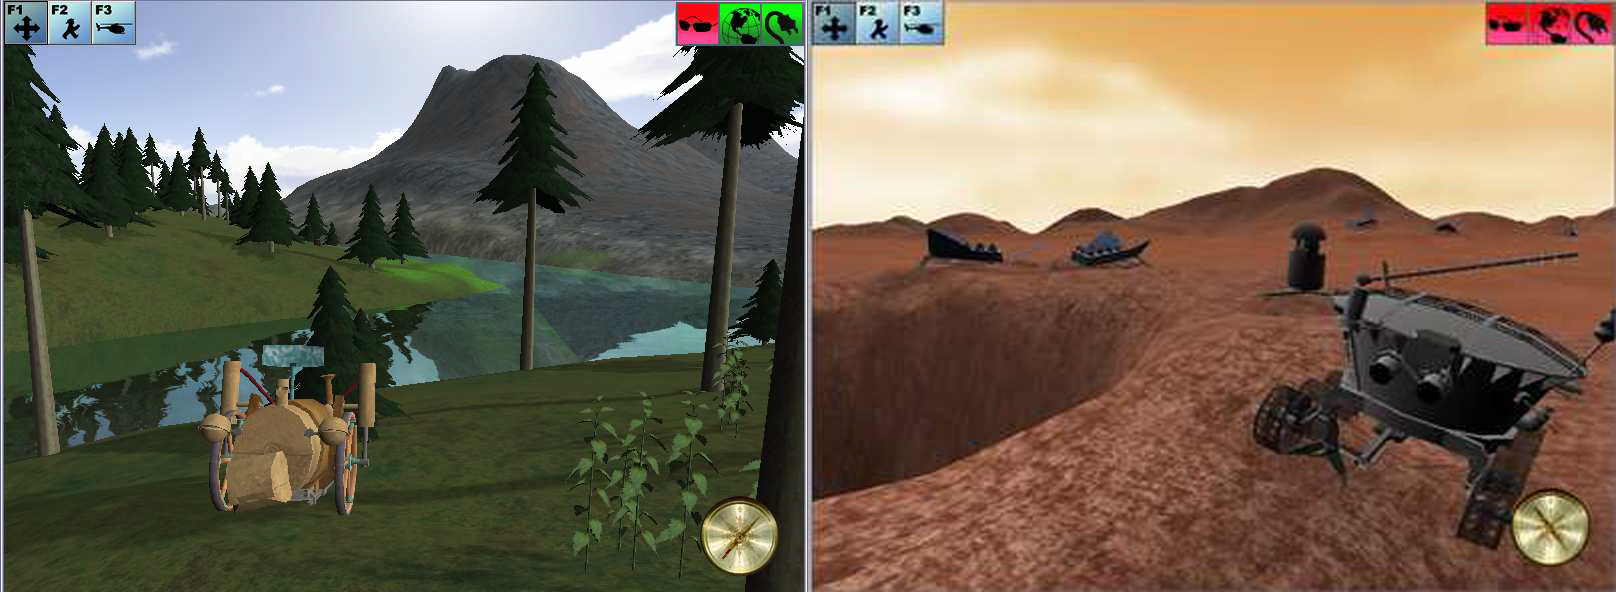
\includegraphics[width=14cm]{graphics/micropsi_3d_screen}
  \caption{Screenshots of the 3D visualisation component in MicroPsi (taken from \cite{Bach:2009:PSI:1611304})}
  \label{micropsi_3d_screen}
\end{figure}

Simulated environments proved especially to serve well for the research of collaborative behaviour of multiple agents, for mapping and exploration, image processing as well as for memory and planning. Additionally, some scenarios, that are almost impossible to implement in the physical world (such as evolving agent populations) could easily be simulated. On the other hand, downsides of simulated worlds include being limited by computing power and the programmer's specifications.~\cite{Bach:2009:PSI:1611304}

    \section{MicroPsi 2}
To ensure broad understandability and to maintain platform independence, MicroPsi has been built ground up again in 2011 and 2012 using more lightweight Python code. What is remarkable about the new implementation called MicroPsi 2 (in the following MicroPsi), is that the simulation is deployed as a web application and the graphical interface is completely rendered inside a web browser, using state-of-the-art internet- and web application technologies.~\cite{conf/agi/Bach12}
        
Even though there have been more complex simulation environments (e.g. 3D-worlds) for previous implementations of Psi architectures, the relatively new version of MicroPsi so far has only two fairly simple ones: a 2D-Island and a map of the public transportation system of Berlin~(see figure~\ref{mp2_berlin}). Instead of building a new 3D-world, with this project we set out for something more experimental. More on this follows in chapters three and four.

\begin{figure}[h]
  \centering
    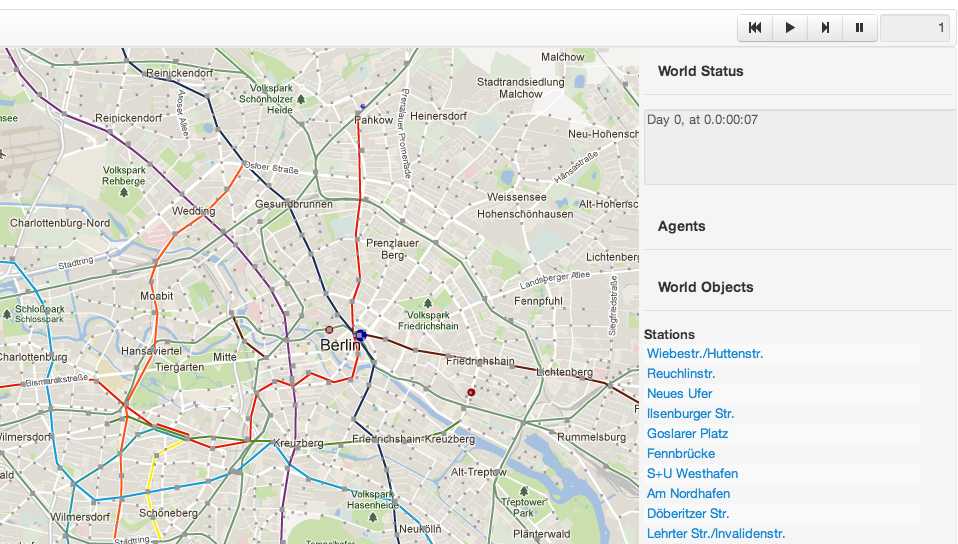
\includegraphics[width=14cm]{graphics/mp2_berlin}
  \caption{MicroPsi's simulation environment Berlin}
  \label{mp2_berlin}
\end{figure}

        \subsection{Module Overview}
    
%TODO Was macht so ein node net? Sollte vorher klar werden!

%TODO Wozu? Bitte nur das beschreiben, was du auch erklärst und brauchst (user & config manager)
        
MicroPsi is written in Python with a minimum of dependencies. Therefore, its  modular structure is comparably easy to understand. It is illustrated in figure~\ref{micropsi2_modules}. First, one can differentiate in between the \texttt{Server} module (or the web interface) and the actual simulation \texttt{Runtime} module (also called \emph{core}). In a simple simulation experiment setup, MicroPsi runs three threads: one for the \texttt{Server} and, invoked by the \texttt{Runtime}, one \emph{world runner} that runs a simulation world as well as one \emph{node net runner} that runs a node net. As these names suggest, the \texttt{Runtime} manages both the simulation environments as well as the inhabitant agents (or node net embodiments). They may by design run asynchronously. In fact, the \texttt{Runtime} works entirely independently of the \texttt{Server} and therefore may just as well be deployed for command line interaction or other GUIs. Furthermore, the \texttt{Server} contains a \texttt{UserManager} and the \texttt{Runtime} a \texttt{ConfigurationManager}.~\cite{conf/agi/Bach12}
\\          

%TODO !! Das ist kein UML. An einem Lehrstuhl für Softwaretechnik sollte es das sein. Außerdem sind nicht alle Module erklärt, sowie die Assoziationen erwas unklar
          
\begin{figure}[h]
  \centering
    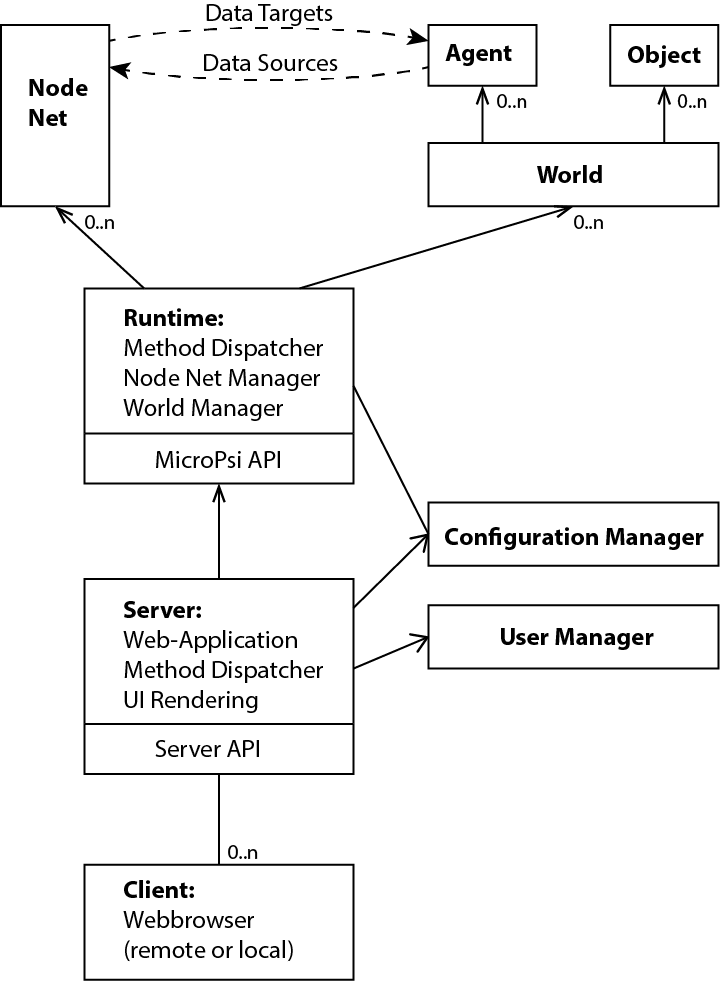
\includegraphics[width=8cm]{graphics/micropsi2_uml}
  \caption{The modular architecture of the MicroPsi framework makes it easy to extend. (taken from~\cite{conf/agi/Bach12})}
  \label{micropsi2_modules}
\end{figure}

The following description is heavily based on \cite{conf/agi/Bach12}, where the theoretical foundations can be found in detail.

        \subsection{Module \texttt{Server}}
The \texttt{Server} renders the GUI and deploys the agent simulation as a web application. It acts as a web server for remote or local access. A client for this application may be any computer with a reasonable up-to-date web browser. Therefore, simulations can be launched from anywhere without requiring any installation. It rests upon the lightweight Python web framework \emph{Bottle}~\cite{bottlepy}.

The web interface is based on HTML as well as Javascript. The communication in between the browser and the simulation is managed via JSON remote procedure calls. Many GUI components of Twitter's \emph{Bootstrap} library are in use. The graphic renderings (see figure~\ref{micropsi2_nodenet}) utilise the JavaScript graphics library \emph{PaperJS}. 

\begin{figure}[h]
  \centering
    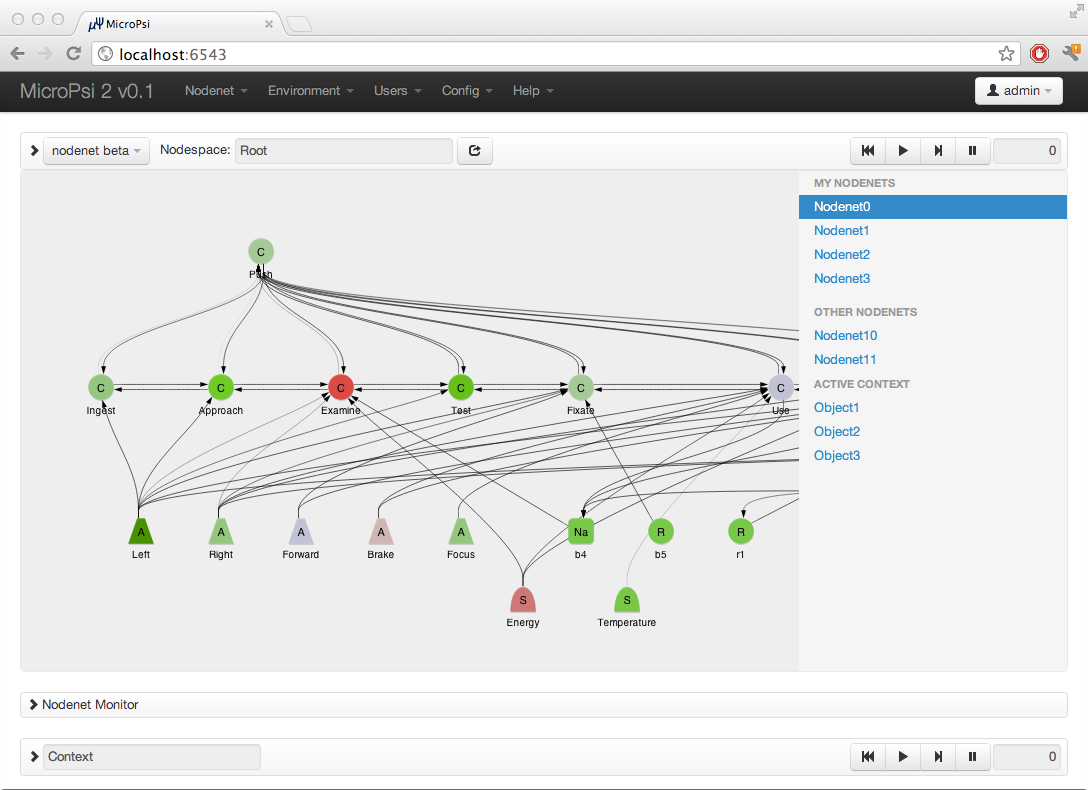
\includegraphics[width=13cm]{graphics/micropsi2_nodenet}
  \caption{The graphical editor is the primary interface to node nets. (taken from~\cite{conf/agi/Bach12})}
  \label{micropsi2_nodenet}
\end{figure}

The \texttt{Server} communicates with its users through the server API. User sessions and access rights are managed by the \texttt{UserManager}.
   
        \subsection{Module \texttt{Runtime}}
In this setup, the \texttt{Server} starts the \texttt{Runtime}---even though it may also work independently of the \texttt{Server}. The \texttt{Runtime} component communicates with the \texttt{Server} through the MicroPsi API. It manages node nets and worlds.

        \subsubsection{Node Nets}

%TODO Wozu knotentypen? wozu benutzt man node nets? Leider verstehe ich das gar nicht
        
A MicroPsi node net is defined as a set of states, a starting state, a network function, that defines how to advance to the next state, and a set of node types. Data sources and data targets serve as the input for nodes and output towards a world, where a data source is filled with data from the world and data targets are linked to agent actions in the world.

According to the Psi theory, nodes may have different types and parameters. They contain gates and slots that send and receive an activation. In most cases, the activation is forwarded from a slot to a gate without further modulation.

Nevertheless, nodes may include functions that enable the creation of new nodes and links as well as procedures for learning and planning. They may be implemented as Python code.

According to the concepts of the Psi theory, MicroPsi defines agents as node nets or to be more specific, hierarchical spreading activation networks. They are an ``abstraction of the information processing provided by brain''~\cite{conf/agi/Bach12}. Agents can be placed and researched in simulation environments or physically embodied as robots.

%TODO cite * 2

%TODO Was willst du damit sagen? Zu kurz!

As node nets share the relevant characteristics with neural networks, they may enable neural learning paradigms. To store information they can form semantic networks. Furthermore, nodes may contain state machines and other operations, which make it possible to build modularised architectures.

        \subsubsection{Worlds}
The simulations worlds are the environments in which we can study our agent's behaviour. Worlds need to provide a world adapter which functions as the interface in between a node net and the environment. Within the world adapter, data sources and data targets have to be defined carefully, to get a functional and meaningful experiment going. They represent the agent's sensory input and the motoric output. Sophisticated interconnection of those enables interaction with the environment.

The kind of data the world adapter interfaces, is not specified any further, which gives developers the opportunity to experiment with classic simulation worlds, as well as exotic applications (eg. stock data). At the time of the original development of the MicroPsi, the prioritised application was building a framework for knowledge representation.

            \paragraph{Objects}$\;$ \\
Worlds contain objects. Objects may be anything that could be interesting for a simulation, and that needs some kind of integrated logic. Light sources or collectable resources are a common example. Objects may contain a set of functions and states, but at least one function that determines how the object advances and reacts to changes while moving through a simulation cycle. A comprehensive world function calls every object function for each simulation step of the world.

            \paragraph{Agents}$\;$ \\
Agents are objects that are connected to a world adapter which makes them controllable by a node net. The object that incarnates the agent is best thought of as the agent's body. The function that advances the agent checks for input from the node net and outputs to it.
        
    \section{Summary}
This chapter provided the necessary foundations regarding AI for this Thesis. It introduced Artificial General Intelligence as a subSet of AI research and presented its main ideas and goals, as well as regarding foundational philosophical questions.
Then, the Psi theory by Dietrich Dörner has been described briefly. An overview of implementations of the Psi theory has been given. The latest framework dedicated to the Psi theory, MicroPsi 2, has been described and it's architecture outlined. Knowing about MicroPsi 2's modules is a necessary foundation for the additions to it that are described in chapter 4.

% !!! An diesem Punkt sollte komplett klar sein, was Psi ist und was von MicroPsi 2 zu erwarten ist. Für Psi reicht die Erklärung bei weitem nicht aus, für MicroPsi vermutlich schon, wenn du Psi Erklärung da ist und mit der Implementierung in Relation gesetzt ist!
\chapter{Minecraft}
\label{chap:3}
To understand how and why the video game Minecraft~\cite{minecraft} is expected to be an interesting simulation environment for artificial general intelligence, necessary background information, about what makes Minecraft different from many other games, has to be given first. To furthermore work with it, the essential components of the game's architecture have to be described. This chapter provides a roundup of Minecraft's history and a brief explanation of the basic game mechanics. They are followed by an overview of Minecraft usages that exceed the original game's purpose as well as an explanation, of why Minecraft is suitable as a simulation environment. Eventually, related software projects, that have been used for this thesis are introduced and described.

    \section{Overview}
The story of Minecraft has many interesting sides, but first and foremost it is a story of immense, unexpected success. To give an overview of it, this section delivers insights into its central ideas, as well as a general look upon the developer's practices. Moreover, the game's reception is considered, as the game has become unusually popular. The descriptions are based on Sean C. Duncan's article \emph{Minecraft, beyond construction and survival}~\cite{Duncan:2011:MBC:2207096.2207097}.
    
        \subsection{Main Ideas}
When Markus (``Notch'') Persson built and released the first public version of Minecraft, it soon became apparent that his creation resonated with many people. The simple concept of a world entirely consisting out of standard sized building blocks, which the player can create, destroy and relocate one-by-one, enabled many gamers to employ their creativity, explore the Minecraft world and test out its possibilities and boundaries.

Looking at the game for the first time, it is impossible to oversee the primitive appearance of its graphics engine. Everything in the game is made out of blocks. May it be the leaves of a tree, dirt, people or the clouds. Even the sun does not appear round, but as a cubic object. One can assume that the obvious connotation to Lego\texttrademark~is more than a coincidence, as it immediately gives the player a clue, about what kind of possibilities for building and creating the game might deliver.

Another interesting aspect about Minecraft is the procedural semantics the game world is generated with. Trees in Minecraft, for example, may share a similar structure that consists of a trunk and leave-covered branches spreading out fractally, but the particular characteristics of each tree are generated randomly. This makes a Minecraft world somewhat more realistic than those of many other videogames.

Minecraft strives to be the opposite of a game with a strict game-flow. Instead, it enables the player's creativity and joy of creation.

        \subsection{Development Process}
The development process of Minecraft is very different from those of most other well-known games. Instead of building the game over months or years to finally release a (more or less) finished version to the public, Minecraft is being designed iteratively. In fact, Persson released the first version only a week after he started working on the game. Ever since, new features have been added, and new versions of the game have been released frequently. Another defining aspect of the game's developement studio Mojang's approach towards the development of Minecraft is the involvement of the game's players. Since the earliest stages, plans for the game's future have been discussed openly, and many times the players' voices have been heard. Persson himself locates his approach in the field of agile software development.~\cite{Duncan:2011:MBC:2207096.2207097}

        \subsection{Reception}
The game has attracted great attention ever since its first release in 2009. Since copies of the game could be obtained commercially for the first time, its different versions sold more than 26 million times---with the PC version priced at 19.95\euro, for example. It should be noted that Minecraft's development studio Mojang is a so called \emph{indie game developer}, that is not associated with any classical game publisher, but distributes copies of their game exclusively via their own website.

Minecraft can certainly be called a world wide phenomenon. The game's developers received a number of prizes for their creation---not to mention the millions of dollars that have been earned in Minecraft sales. With its huge success, Minecraft has proven clearly that it compelled to many players.

Unlike any other game, Minecraft fosters the creativity of its players. Bringing the construction component to one extreme after the other, well publicised player creations include a life-size model of the USS Enterprise-D as well as a fully functional arithmetic unit. Videos of roller coaster rides through complex constructions increasingly show characteristics of an art form themselves---regarding to the amount of views on youtube, not less than other, well established formats.

    \section{Game Mechanics}
Now knowing about the game's background, in this section we will continue with descriptions of the basic concepts of the game, that regard to our AI interface. 

Before a new Minecraft game begins, it procedurally generates a three-dimensional world. The player is then dropped to a spawn point and is now facing a scenario and a minimal game interface, lacking any kind of instruction or advise about what to do next. Soon, the procedurally generated world drives most players to explore the highest mountains and deepest caverns. As the player collects resources and crafts items, resources harder to reach and items more complex to craft become available.~\cite{Duncan:2011:MBC:2207096.2207097}

Although the game can be downloaded and played as a single packet of software, many scenarios of playing the game consist of running a Minecraft server software, as well as one copy of the client software for each player. It is possible to mimic the official client by implementing the reverse-engineered client-server-protocol and therefore build artificial players that way.

The structure of Minecraft worlds and the client-server-protocol are described in the following. The descriptions are based on the regarding articles of the \emph{Minecraft Wiki}~\cite{mcwiki}.

    \subsection{Minecraft Worlds}
    
%TODO Gibt es irgendwelche Optionen für dieses Paket, damit die Figure 3.1 linksbündig angezeigt wird?

\begin{wrapfigure}{l}{0.3\textwidth}
  \begin{center}
    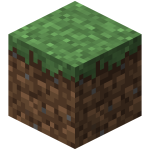
\includegraphics[width=0.15\textwidth]{graphics/block}
  \end{center}
  \caption{A grass block (CC-BY-3.0 Mojang AB) \cite{image_mob}}
  \label{mc_block}
\end{wrapfigure}

The most significant concept in Minecraft is the block~(see figure ~\ref{mc_block}). A block is a cube which sides are, compared to the player, roughly one meter long. Every Minecraft world is built up entirely out of them. Therefore, worlds can be thought of as three dimensional spaces filled with voxels.~\cite{baloghcodemetropolis} There are many different types of blocks (or materials, they consist of) and they share their single size, which converts to the basic distance unit of Minecraft.

A chunk~(see figure ~\ref{mc_chunk}) is a segment of the Minecraft world that is 16 blocks long, 16 blocks wide and 256 blocks high (or deep) and therefore consists of up to 65,536 blocks.~\cite{mcwiki_chunks}

\begin{wrapfigure}{r}{0.15\textwidth}
  \begin{center}
    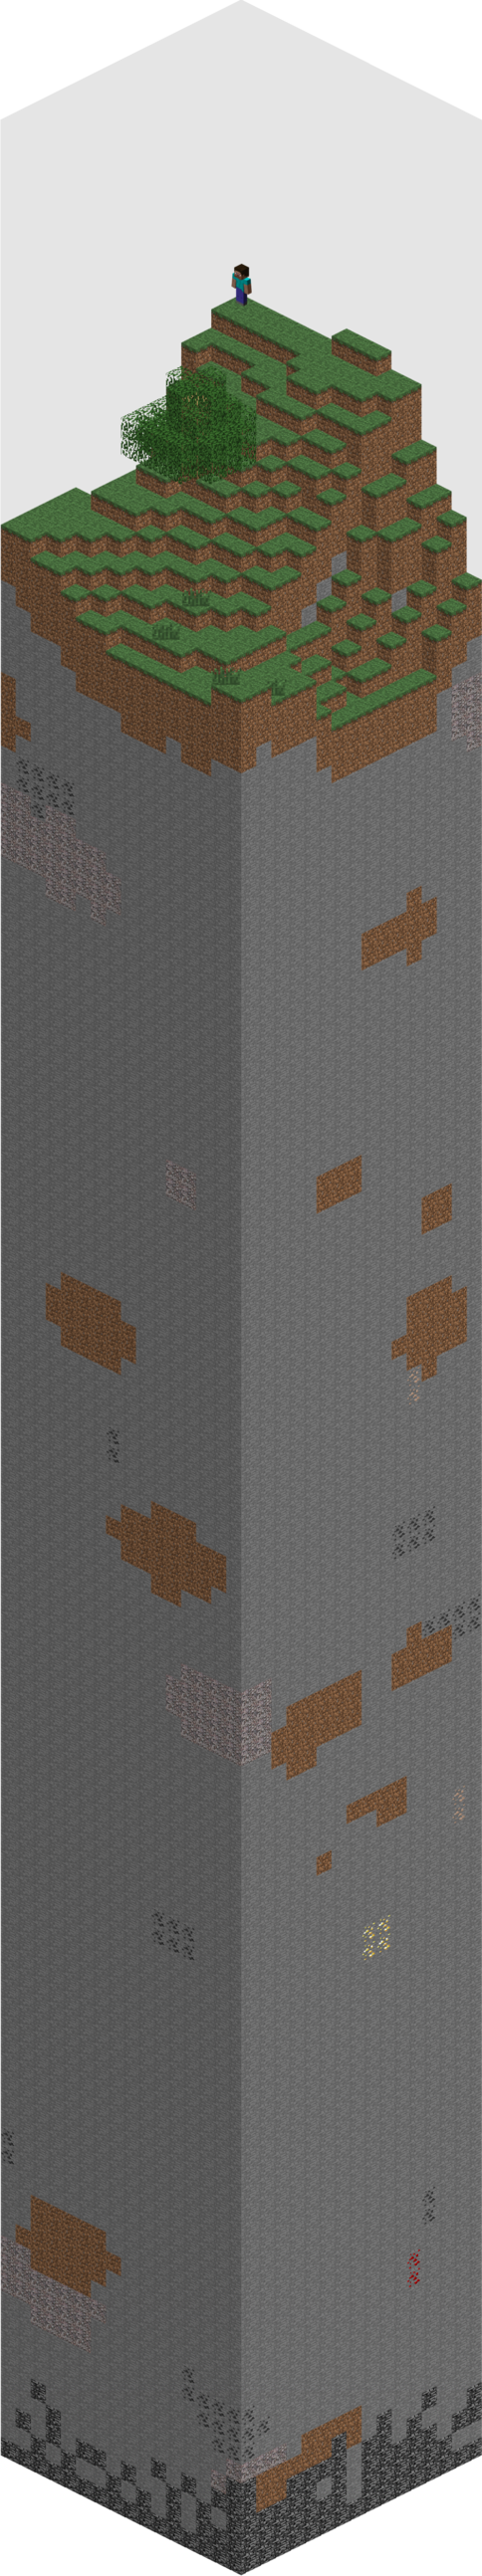
\includegraphics[width=0.16\textwidth]{graphics/chunk}
  \end{center}
  \caption{A chunk (CC-BY-3.0 Mojang AB) \cite{image_mob}}
  \label{mc_chunk}
\end{wrapfigure} 

"The player"~(see figure ~\ref{mc_player}) is what the playable game-character in Minecraft is called. It is usually displayed as a human.
Also, a Minecraft world has a day-night-cycle with 24 Minecraft hours converting to 14 minutes by default.

\begin{wrapfigure}{l}{0.3\textwidth}
  \begin{center}
    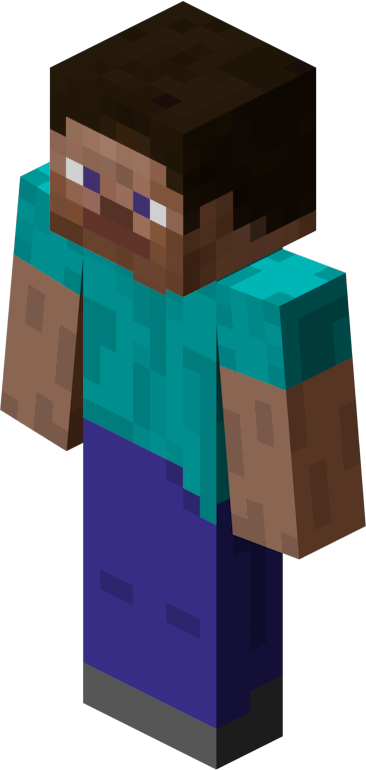
\includegraphics[width=0.06\textwidth]{graphics/player}
  \end{center}
  \caption{The player (CC-BY-3.0 Mojang AB) \cite{image_mob}}
  \label{mc_player}
\end{wrapfigure} 

The game itself has no predefined goals. Players can walk around, discover the created world (see figure \ref{mc_mechanics} 1) and collect resources by \emph{destroying} blocks, with the generated resources equaling the block type. They can combine several resources to \emph{craft} items. For example, a player can destroy the blocks that represent a tree~(see figure \ref{mc_mechanics} 2). The gained \emph{wood} resource could then be used to craft a wooden pickaxe~(see figure \ref{mc_mechanics} 3), which could then be used to dig into the ground more efficiently~(see figure \ref{mc_mechanics} 4) to then \emph{mine} more rare resources, like iron or gold.

There exist different game modes. The original \emph{survival} mode adds monsters that attack the player at night. What solutions to survive the player comes up with (e.g. building shelter or fighting the monsters) is left up to him or her.

In \emph{creative} mode, the player is not being attacked by monsters, has the ability to fly and is given instant access to unlimited resources.

The mode of a Minecraft world does not effect the functionality of this project.

\begin{figure}[h]
  \centering
    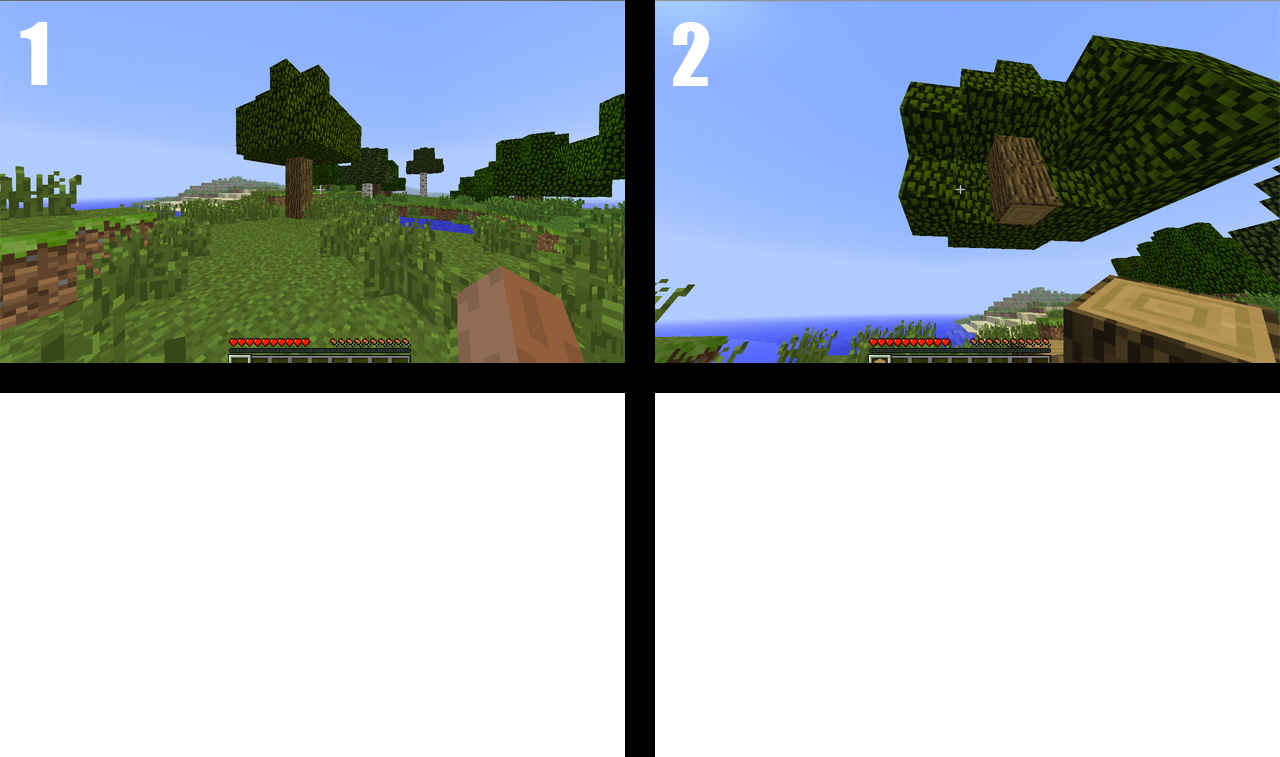
\includegraphics[width=15cm]{graphics/minecraft_mechanics}
  \caption{Screenshots of Minecraft's basic game mechanics}
  \label{mc_mechanics}
\end{figure}

        \subsection{The Client Server Protocol}
        \label{client_server_protocol}
Minecraft's client server protocol is not publicly documented by the developers themselves. However, the modding community gathered comprehensive knowledge and understanding of its structure (probably by using reverse engineering techniques). The protocol is based on packets. 

The NBT (Named Binary Tag) is a data format that has been introduced by Persson to transfer chunks of binary data together with small amounts of additional data. Its main use is to store Minecraft worlds.

Packets are either \emph{server to client}, \emph{client to server} or \emph{two-way} and begin with a \emph{packet ID} byte. The structure of the packet's payload depends on it's packet ID.
 
To give an example of one of the easier packets, the \emph{Client Position} packet is fairly straightforward~(see table~\ref{mc_packet}). It is exclusively send from clients to servers and starts with its packet ID (as every packet does), followed by the X- and Y-coordinates as doubles, the stance value as a double (which is used to modify the player's bounding box), another double for the Z-coordinate and eventually a boolean that describes if the player is on the ground or not.~\cite{protocol}

\begin{table}[htb]
\centering
\begin{tabular}{|c|c|c|}\hline

    Field Name & Field Type & Notes \\ \hline
   Packet ID & Byte & 0x0B \\ \hline
   X & double & Absolute position \\ \hline
   Y & double & Absolute position \\ \hline
   Stance & double & Used to modify the players bounding box \\ \hline
   Z & double & Absolute position \\ \hline
   On Ground & boolean & Derived from packet 0x0A \\ \hline
   
\end{tabular}
\caption{The structure of the packet ``Player Position (0x0B)''~\cite{protocol}}
\label{mc_packet}
\end{table}

Knowledge of this data structure is already sufficient to move around in the Minecraft world. To go forward, one has to figure out the players current position, calculate the absolute coordinates of the destination of the movement in regard to it and send a Client Position packet with these coordinates via a TCP socket to the server. If the destination is not more than 100 blocks away from the origin of the movement, the server accepts the movement. In the official Minecraft client, a player's movement from one point to the other is rendered with a walking animation.

Other than movement, packet structures are defined for every aspect of the game. May it be the initial handshake, the creation or destruction of blocks or activities of other player- or non-player-characters.

This protocol is what a custom Minecraft client needs to speak.

    \section{Minecraft as a Gaming Platform}
With more and more applications that move beyond the original gameplay of construction and survival, Minecraft seems to shift gradually towards being not only a game, but also a gaming platform, that many other people use to implement their own ideas. Inside Minecraft worlds, players have created games for educational purposes, for example. A group of students of the Miami University developed a game called Circuit Magic that is committed to teaching the players about logical circuits. The famous Minecraft Teacher, who implements Minecraft in primary school classes, is another good example. Following in his footsteps, ``Massively Minecraft'' is a community of teachers who share their thoughts and experiences with doing the same. Just as well, games have been developed for the purpose of artistic expression. Chain World, the game that tried to simulate religion, is an exciting example. Not only do players implement their engagement inside Minecraft. The internet is full of Minecraft content, be it videos on Youtube, online tutorials or other community based knowledge resources, headquartered at the Minecraft Wiki\footnote{\url{http://www.minecraftwiki.net/}}.~\cite{Duncan:2011:MBC:2207096.2207097}

As user-generated content has been an essential part in the development of Minecraft, in a process that reminds one of a self-fulfilling prophecy, more and more people explore its possibilities to experiment with new applications. As of today, Persson and Mojang seem to favour and approve new uses of their creation.~\cite{Duncan:2011:MBC:2207096.2207097}

    \section{Suitability of Minecraft as a Simulation Environment}
There are a number of reasons why using Minecraft as a simulation environment could be useful and lead to interesting results.

First, the game itself is easily accessible. It is developed using Java (for both the client and the server software) and, therefore, up to a certain extend, platform independent. The desktop computer version is being sold for Windows, Mac OS X and Linux devices. There are official ports for Android, iOS, Xbox 360, the Raspberry Pi and a version for the upcoming gaming console Xbox One is announced. The desktop versions are priced at 19.95 \euro, which make it affordable to a large audience.

The game itself already has an enormous fanbase. It is (like most videogames) especially popular among teenagers. Minecraft being loved by so many people could benefit this project, in terms of leading to increased attention.

The game's developer has proven many times that it acts generously towards  other developers, when it comes to the creation of game modifications and content that builds upon or changes original Minecraft intellectual property. As mentioned before, Mojang is not restrictive towards users doing all kinds of things with their creations. This led to the availability of a fairly complete community-sourced  documentation and explanation of virtually every aspect of the game---including its software architecture, data structures and protocols. This is useful for this project, as chances are low that they will have anything against using Minecraft for AI simulations in the foreseeable future. To the contrary, the game's AI creator Jon Kagström provided advise for this project

The Minecraft world, with its logic, semantics and functionalities, offers possibilities for an AI to prove being able to interact with the environment---in primitive ways (e.g. moving around), as well as with increasingly complex tasks like building, collecting resources, crafting items and interacting appropriately with both well-disposed and hostile other entities.

The semantics of the gameworld share characteristics with the real world. Moving through a Minecraft environment, one quickly realises that the game has generated different biomes (eg. forest or tundra). Also, trees, rivers, mountains and ore veins are neither hard-coded nor appear completely random, but are generated procedurally and their structure appears to be (somewhat) fractal.
        
Using Minecraft as a simulation environment will give Psi agents possibilities to show off, what kind of sophisticated behaviour they are capable of.

    \section{Related Projects}
    \label{sec:3:relatedprojects}
Minecraft's success inspired many other projects, including artificial players and a number of Minecraft-like games in a wide variety of programming languages and environments.


        \subsection{Minecraft Bots}
There exist many projects that could be considered Minecraft \emph{bots}. One has to differentiate in between two types. On the one hand, there are those that mimic an entire client software and facilitate communication with the server on the default client software's behalf. On the other hand, there are bots which are modifications of the original client (or server) software and usually add non player characters---like animals and other non-human creatures---to the game. The code is usually injected through one of the popular \emph{modloaders} (e.g. Minecraft Forge).

One example (and probably the most advanced one) for an entire bot framework that replaces the client, is \emph{Mineflayer}~\cite{github_mineflayer}. It has a high-level abstraction of the environment (eg. entity knowledge and tracking) and is written in JavaScript using node.js. However, it has not been used for this project, because a Python implementation was aimed for, as it is explained in the next section.

Opposed to Mineflayer, an example for game modification bots are the \emph{Cubebots}~\cite{mcforums_cubebot}---fan-made non-player characters that aim to help Minecraft players with mundane tasks.

Most third party clients, including bots, facilitate their own event loops. 

    \subsubsection{\texttt{Spock} by Nick Gamberini}
Developed by Nick Gamberini, \texttt{Spock}\footnote{\url{https://github.com/nickelpro/spock}} is an open-source bot framework (and as such also a Minecraft client) written in Python. It has been chosen to become an essential part of this project for two reasons: being written in Python it painlessly integrates in the existing MicroPsi code and the absence of dependencies (with one exception) leave the code understandable and easy to deploy.
    
    \subsubsection{Protocol Implementation in \texttt{Spock}}
    
%TODO zu kurz! Erklärung fehlt
    
The Minecraft protocol implementation in \texttt{Spock} is straightforward. The necessary data structures are stored separately and can be accessed globally (see figure~\ref{snippet_structures}).

		
		\begin{figure}[ht]
			\centering
			\begin{minipage}{8cm}
				\begin{pseudocode}
names = {
	0x00: "Keep Alive",
	0x01: "Login Request",
	0x02: "Handshake",
	0x03: "Chat Message",
	...

structs = {
	#Keep-alive
	0x00: ("int", "value"),
	#Login request
	0x01: (
			("int", "entity_id"),
			("string", "level_type"),
			("byte", "game_mode"),
			("byte", "dimension"),
			("byte", "difficulty"),
			("byte", "not_used"),
			("ubyte", "max_players")),
	...
					\end{pseudocode}
				\caption{An excerpt of \texttt{Spock}'s data structures for packet-IDs and -structures}
				\label{snippet_structures}
			\end{minipage}
		\end{figure}
		
These structures are used to parse each packet appropriately (see figure~\ref{snippet_parse}).

		\begin{figure}[ht]
			\centering
			\begin{minipage}{13cm}
				\begin{pseudocode}
def decode(self, bbuff):
	#Ident
	self.ident = datautils.unpack(bbuff, te')
	
	#Payload
	for dtype, name in ta.structs[self.ident][self.direction]:
		self.data[name] = utils.unpack(bbuff, dtype)
					\end{pseudocode}
				\caption{\texttt{Spock}'s function for decoding packets}
				\label{snippet_parse}
			\end{minipage}
		\end{figure}
		
		\subsection{Minecraft Clones}
Other interesting projects include Skycraft~\cite{skycraft}, a Minecraft-like browser game based on WebGL. Another particular project that has the same name as the original game that inspired it is \texttt{Minecraft} by Michael Fogleman~(see figure~\ref{fogleman_mc_screen}). It is a simple Minecraft clone in under 600 lines of Python and has gained some popularity on reddit~\cite{fogle-reddit} and Hacker News~\cite{fogle_hn}. It is comparably easy to understand and modify and has been used for the visualisation component of this project. It is based on the Python multimedia library \emph{Pyglet}~\cite{pyglet}.

\begin{figure}[h]
  \centering
    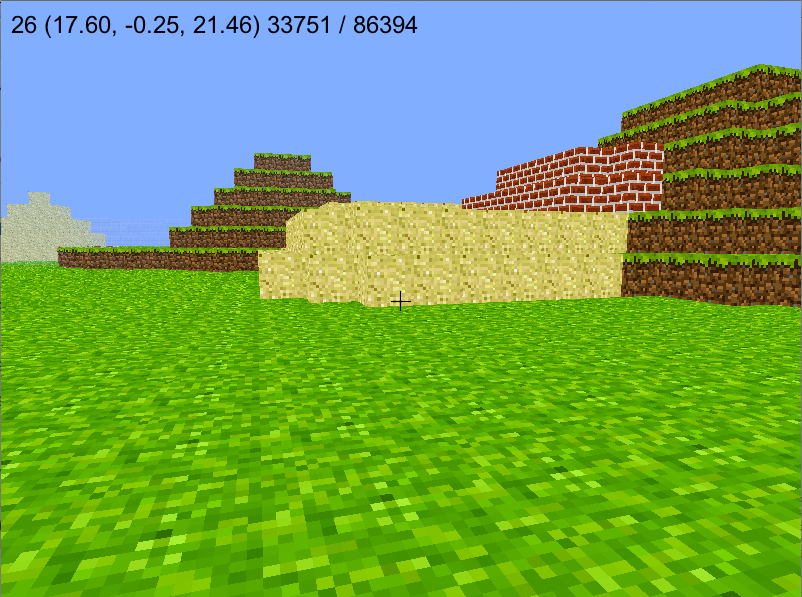
\includegraphics[width=10cm]{graphics/fogleman_mc_screen}
  \caption{A screenshot of \texttt{Minecraft} by Michael Fogleman}
  \label{fogleman_mc_screen}
\end{figure}

    \section{Summary}
An overview of Minecraft, its history and its basic concepts, as well as other software in its periphery, have been presented in this chapter. Minecraft is a complex, yet easily accessible virtual world. It is in constant development and new features are added regularly. It has a massive fanbase and a huge community around all kinds of game modifications. The most important concepts of Minecraft for this thesis are blocks, chunks and also the client server protocol. They will all be used in the next chapter.
As a basis for the implementation of the Minecraft interface for MicroPsi, the bot framework \texttt{Spock} by Nick Gamberini has been chosen to extend MicroPsi.
Furthermore, \texttt{Minecraft} by Michael Fogleman has been chosen to serve as a foundation for the visualisation component. Their implementations will be presented in detail in the next chapter.

%TODO Warum hast du Minecraft ausgewählt? API öffentlich zugänglich, passende Erweiterungen vorhanden, eigenständig erweiterbar, Welt wird realitätsnah nachgebildet
\chapter{A! Approach / Minecraft as a Simulation Environment for MicroPsi 2}

The objective of this thesis is to build and test an interface in between MicroPsi and Minecraft, so that a Minecraft world (e.g. server) can be used as a simulation environment for the MicroPsi 2 Framework, which will act as an artificial player.

The modular architecture of MicroPsi 2 allows it to add new simulation environments (or worlds, as they are called in microPsi) fairly easy. A world needs interfaces to Data Source and Data Targets and a step-function that evolves the world.

That being said, a big part of the project is about visualization. Inside the MicroPsi Core Application, a 3D-visualization of the Minecraft world and the agent within is aimed for. There are two main reasons for this goal. The first reason is, that the agents behavior within the simulation environment is supposed to be monitored from the MicroPsi webinterface in an aesthetically appealing way. The secons reason is, that the image data is supposed to be processed by the agent as one of it's senses.

The functionality is to be tested with a simple Braitenberg-vehicle experiment.

Do obtain these goals, the Minecraft Client-Server-Protocol had to be researched, learned and imitated.

Then, artificial Minecraft players (written in Python) had to be searched, found and researched.

Eventually, building upon an existing Bot framework led to an integration with the MicroPsi framework.

\section{A! Overview / What has been there so far?}
... Minecraft Bots with simple as well as sophisticated AI ...
... MicroPsi 2 with Island and Berlin world ...

\section{A! Architecture / Building the interface in between Minecraft and the simulation environment}
... result: a Minecraft Bot that implements MicroPsi AI and is controlled and monitored via the MicroPsi webinterface ...
... the Webinterface holds its own visualization of the Agents worldview ...

\subsection{A Minecraft Bot}

\subsubsection{Protocol Implementation}

\subsubsection{Control Structures}

\subsubsection{Previous own implementations with TwistedBot}

\subsubsection{other popular Bot projects and game modifications}

\subsubsection{Spockbot von Nickelpro}

\subsection{Implementing the Bot in MicroPsi}

\subsection{The MicroPsi side}

\subsection{necessary Modifications and Additons in core/worldrunner}

\paragraph{Data Targets and sources}

\subsection{necessary Modifications and Additons in server/control and monitoring interface}

\subsection{The Visualization}

\subsubsection{Requirements and necessity of a visualization}
... why a visiualization and what is it supposed to do? ...

\paragraph{monitoring the bot from the webinterface}
... make it aesthetically appealing as well as easily accessible ...

\paragraph{using visualization output as a Datasource / as the bots eyes}

\subsubsection{Implementation}

\paragraph{used Data}
... required Data for the visualization ...
... and how to obtain it (first attempts: telnets/then sockets) ...

\subsubsection{3D Visualisierung mit Pyglet}
... foundation: that minecraft pyglet clone ...

\subsubsection{Earlier attempts using JavaScript / AJAX}
... worked well but a little slow ...

\section{A! Implementation}
% TODO je nach Größe des Kapitels, das hier vielleicht eine Ebene höher ziehen (versuche dich hier erstmal nur auf die fertige Lösung zu konzentrieren und warum du dich dafür entschieden hast. Es ist nicht interessant, was du sonst alles ausprobiert hast, außer dass du konkret angibst, warum du dich für die jetztige Implementierung im Vergleich zu anderen entschieden hast)

\section{A! Case Study}

\subsection{Experiment}
... experiment to test functionality of the system ...
... scope: only a simple test for time reasons ...

\subsubsection{Braitenberg Vehicle}
... simplest proof of concept of a microPsi agent ...
\chapter{Conclusion}
%Analyse und Zusammenfassung / Auswertung der Ergebnisse / Diskussion der Ergebnisse und weitere Erkenntnisse / Limitationen und Ausblick
After several iterations and trying out different approaches and technologies the Interface is now functional.

The experiment with the simulated Braitenbergvehikel resulted in proofing that Minecraft is usable as a simulation environment.

\section{What's next}
In the future, multiple agents shall interact with the same environment and collaborate with each other.
... what has been learned ...
... what can be done with the new environment ...
... what can be improved? ...
... what other simulation environments could be of interest? ...

% include more chapters

% optional
%\begin{appendices}
	\chapter{Auszug aus dem Buch}
	Beispielhaft wird hier gezeigt, wie Block-Zitate eingeführt werden können. Hier der Beginn des Buchs "`Per Anhalter durch die Galaxis"' von Douglas Adams~\cite{adams1998anhalter_inbook}:
	
	\begin{quote}
	"`Das Haus stand auf einer kleinen Anhöhe genau am Rand des Ortes. Es stand alleine da und überblickte das weite Ackerland im Westen. Absolut kein bemerkenswertes Haus - es war ungefährt dreißig Jahre alt, plump, viereckig, aus Ziegelsteinen erbaut und hatte vier Fenster an der Vorderseite, der es nach Größe und Proportion mehr oder weniger mißlang, das Auge zu erfreuen."'
	\end{quote}
	
	\chapter{Implementierungen}
	Beispielhaft wird hier gezeigt, wie Code-Beispiele in den Text eingefügt werden können. Die Pseudocode-Umgebung wird von \emph{macros.tex} bereitgestellt und kann dort entsprechend angepasst werden.
			\begin{figure}[ht]
			\centering
			\begin{minipage}{11cm}
				\begin{pseudocode}
public static Object answeringMachine() {
	Thread.sleep(1000);
	return 42;
}
				\end{pseudocode}
				\caption{Implementierung einer Maschine zur Beantwortung der Fragen aller Fragen.}
				\label{IMG_PID}
			\end{minipage}
		\end{figure}
	
\end{appendices}

\backmatter % Do not move this command!

% optional
\phantomsection
\addcontentsline{toc}{chapter}{List of Figures} % change according to language (adds the list of figures to the table of contents)
\listoffigures

% optional
\listoftables
\phantomsection
\addcontentsline{toc}{chapter}{List of Tables} % change according to language (adds the list of tables to the table of contents)

% change according to language
\chapter{Contents of the CD}
The attached CD contains the following::
\begin{itemize}
	\item this bachelor thesis in PDF format,
	\item the Python project MicroPsi including the Minecraft world adapter,
	\item the binaries of a Minecraft server that can be used to test the implementation.
\end{itemize}
%%%%%%%%%%%%%%%%%%%%%%%%%%%%%%%%%%%%%
%%%%%%%%%%%%%%%%%%%%%%%%%%%%%%%%%%%%%

\cleardoublepage
\phantomsection
\addcontentsline{toc}{chapter}{Bibliography} % change according to language (adds the bibliography to the table of contents)
%\bibliographystyle{alphadin} % select this for a German thesis
\bibliographystyle{alpha} % select this for an English thesis
\bibliography{thesis}


\end{document}